%%%%% Document Setup %%%%%%%%

\documentclass[10pt, twocolumn]{revtex4}    % Font size (10,11 or 12pt) and column number (one or two).

\usepackage{times}                          % Times New Roman font type

\usepackage[a4paper, left=1.85cm, right=1.85cm,
 top=1.85cm, bottom=1.85cm]{geometry}       % Defines paper size and margin length

\usepackage[font=small,
labelfont=bf]{caption}                      % Defines caption font size as 9pt and caption title bolded


\usepackage{graphics,graphicx,epsfig,ulem}	% Makes sure all graphics works
\usepackage{amsmath} 						% Adds mathematical features for equations

\DeclareMathOperator{\sech}{sech}		% Defining sech so it doesn't italicise it 
\DeclareMathOperator{\Int}{Int}		% Defining 'integer part of' so it doesn't italicise it 
\providecommand{\e}[1]{\ensuremath{\times 10^{#1}}} %shorthand for scientific notation

\usepackage{etoolbox}                       % Customise date to preferred format
\makeatletter
\patchcmd{\frontmatter@RRAP@format}{(}{}{}{}
\patchcmd{\frontmatter@RRAP@format}{)}{}{}{}
\renewcommand\Dated@name{}
\makeatother

\usepackage{fancyhdr}


\pagestyle{fancy}                           % Insert header
\renewcommand{\headrulewidth}{0pt}
\lhead{L. P. Flower}                          % Your name
\rhead{Collisions of Matter-Wave Solitons in a Bose-Einstein Condensate}            % Your report title               

\def\bibsection{\section*{References}}        % Position reference section correctly


%%%%% Document %%%%%
\begin{document}                     


\title{Collisions of Matter-Wave Solitons in a Bose-Einstein Condensate} 
\date{Submitted: \today{}}
\author{L. P. Flower}
\affiliation{\normalfont Durham University L3 Computing Project \\ Project Tutor: Dr. Rahul Sawant}

\begin{abstract}              
 
In this project, the split-step Fourier method was used to propagate bright matter-wave solitons in Bose-Einstein condensates, achieving $<0.01\%$ probability leakage. The simulation was then used to investigate the properties of soliton collisions, both in the free case and in a harmonic trap. Good agreement was found with theory, including the observation that colliding solitons in antiphase results in the solitons appearing to bounce off one another. A classical particle model was introduced where the weak inter-soliton potential was set to zero. The limits of this model were investigated; it was found that for typical experimental timescales, this particle model is excellent when the soliton dynamics are regular and the solitons remain well-separated. However, the non-interacting particles cannot reproduce the phenomenon of bound states of solitons, nor of chaotic dynamics when three solitons are considered. In these cases, the interactions between solitons must be taken into account. Nevertheless this particle model is a useful visualisation tool to appreciate the beautiful chaotic motion of solitons in weakly bound states.  

\end{abstract}

\maketitle
\thispagestyle{plain} % produces page number for front page


%%%%%%%%%%%%%%%%%%%%%%%%%%%%%%%%%%%%%%%%%%%%%%%%%%%%%%

\section{Introduction and Theory} \label{Intro}

Solitary waves or solitons occur in systems where non-linear effects exactly cancel the dispersion of a wave packet, meaning it propagates without changing its shape. Even after collisions with other solitons, these waves emerge with their velocities and shapes unchanged, though a phase shift is imparted to both solitons. Non-linear wave systems are found in water waves, optical fibres and atomic Bose-Einstein condensates (BECs). The latter are described to a good approximation by the non-linear Schr\"{o}dinger equation when the radial confinement of the BEC is good enough that the motion is approximately one-dimensional. 

To describe the behaviour of a Bose-Einstein condensate, an effective potential term $g |\psi|^2$  is introduced into the Schr\"{o}dinger equation to characterise the interactions between the constituent particles. The resulting non-linear Schr\"{o}dinger equation is given by 
\begin{equation} \label{NLSE}
i \hbar \frac{\partial \psi}{\partial t} = -\frac{\hbar^2}{2m} \frac{\partial^2 \psi}{\partial x^2} + (V+g |\psi|^2) \psi,
\end{equation}
where $V$ is the external potential and $|\psi|^2$ represents the density of particles. $\psi$ is normalised such that the integral over all space gives $N$, the number of particles in the soliton system. Describing the interparticle interaction by the pseudopotential approximation $g |\psi|^2$ is valid in the dilute limit, where the average spacing between gas particles is greater than the scattering length, $|a_s|$. 

The solutions to the non-linear Schr\"{o}dinger equation come in two forms. If the interactions are repulsive, i.e. the scattering length between atoms is positive, the interaction parameter $g$ is positive and hence the solutions are 'dark solitons': atom density minima which move without changing shape. But if the interactions are attractive (negative scattering length), the solutions are bright matter-wave solitons with negative $g$, where the centre of a soliton corresponds to a maximum atomic density. In this report we will consider bright solitons only. These can be produced either with a BEC of atoms with an intrinsic negative scattering length, or by tuning the interactions using a Feshbach resonance \cite{Feshbach}. 

To simplify the form of the solutions, it is useful to work in dimensionless units of space and time. A characteristic soliton length $\xi$ can be defined such that on length scales longer than $\xi$, atoms move collectively (as a recognisable soliton) while on shorter length scales, they behave as free particles. Here the soliton length is defined as $\xi = \frac{\hbar^2}{mg}$ \cite{Cornish}. Using the transformations \cite{Transforms} 
\begin{equation} \label{transforms}
x = \tilde{x} \frac{\xi}{\sqrt{2}}, \quad		 t = \tilde{t} \frac{m \xi^2}{\hbar}, 	\quad \psi = \tilde{\psi} \frac{1}{\sqrt{\xi}}
\end{equation}
%\quad inserts quadruple space
to rescale quantities in the nonlinear Schr\"{o}dinger equation, the Gross-Pitaevskii equation (GPE) in its dimensionless form is obtained \cite{Gross} \cite{Pitaevskii}
\begin{equation} \label{GPE}
i \frac{\partial \tilde{\psi}}{\partial \tilde{t}} = -\frac{\partial^2 \tilde{\psi}}{\partial \tilde{x}^2} + (\tilde{V}+g |\tilde{\psi}|^2) \tilde{\psi},
\end{equation}
where the tilde symbols denoting the transformed quantities are omitted for the rest of this report, for clarity of reading. 

The integrable solutions to the Gross-Pitaevskii equation are $\sech$ solitons. A parameter to characterise width, $\zeta$, can be defined with units 1/length. The normalised initial wavefunction is then 
\begin{equation} \label{soliton}
\psi(x) = \sqrt{\frac{\zeta}{2}} \sech{(\zeta x)} e^{i (v x + \phi)},
\end{equation}
where $v$ is the velocity of the soliton and $\phi$ is a phase factor. In order for the soliton to propagate without change of shape, it is required that $g=-4\zeta$. This is found by substituting the $v=0$ case into the time-independent nonlinear dimensionless Schr\"{o}dinger equation and setting $E$ to be $\zeta^2$ to find the stationary-state condition. It is predicted that if the value of $g$ found to confine the soliton in this simulation differs from $-4\zeta$, it is due to the treatment of space and time as discrete variables rather than continuous. 

To check that the length scales of this simulation are suitable for modelling solitons as a collective, we express the interaction parameter $g$ in terms of the parameters of the experimental system. A Bose-Einstein condensate of Rubidium-85 atoms hs been chosen, which has an intrinsic scattering length of $a_s = -0.6$ nm and 2000 atoms per soliton \cite{ExpParams}. The radial confinement has frequency $\omega_r = 2\pi \times 17.5$ Hz. Note that the radial confinement has been assumed to be perfect in the computational part of this project, such that the BEC can be treated as one-dimensional; the axial confinement, if present, is explicitly dealt with in this simulation. The interaction parameter can be written as $|g| = 2\hbar \omega_r |a_s| N$ \cite{Cornish}. Using these realistic experimental figures, $g = -2.78 \e{-38}$ kg m$^3$ s$^{-2}$, where the negative sign comes from the fact we are considering bright solitons. The characteristic soliton length is then $\xi = 2.82 \mu$m. A single unit of rescaled length is equivalent to $\xi/\sqrt{2} = 1.99 \mu$m and box lengths between 20 and 40 rescaled space units are used in this model, hence the length scales are suitable for modelling the behaviour of solitons. In the graphs in this report, the unit of time has also been multiplied by 10 to improve readability. The unit of time displayed on graphs is therefore equal to 0.00107 s, so the simulation was run for at least 0.0214 s and up to 0.128 s. Most experiments are run over the course of $\sim$ 35 ms, around the same order of magnitude as this computational model. 

The name 'solitons' for solitary waves originates from the fact that their dynamics are (largely) unchanged after collisions with other solitons, playing on the usual nomenclature for particles where their names end in '-on'. Throughout the history of solitons, in both water and optical systems, a classical particle model has been useful for describing their motion in applications where the details of collisions are unimportant. An adaptation of the particle model for matter-wave solitons in Bose-Einstein condensates was developed recently \cite{Martin}. The particles are placed in the same external potential $V$ as the solitons, and an effective inter-soliton potential 
\begin{equation}
V(q_j - q_k) = -\eta \sech^2{\eta(q_j - q_k)}
\end{equation}
is a valid approximation when the solitons have equal effective masses $\eta$. $q_i$ is the position of soliton $i$ as a function of time. This potential does not describe the interference effects produced when solitons collide, since classical particles do not exhibit wave-like properties, so it is only a good descriptor away from collision sites. But for soliton separations greater than $2/\eta$, the attractive potential is extremely weak. As a result, if the average soliton separation is greater than $2/\eta$, the inter-soliton potential can be approximated as zero. This will not allow for the formation of bound states of particles, as can occur with real solitons \cite{Bound} and will have impacts on the frequency of collisions when the particles are confined in a harmonic trap. The validity of this approximation will be investigated in this project. 

%%%%%%%%%%%%%%%%%%%%%%%%%%%%%%%%%%%%%%%%%%%%%%%%%%%%%%%

\section{Methods} \label{Methods}

The split-step Fourier method is a mathematical trick borrowed from optics and relies on the fact that in Fourier space, the operator $\frac{d}{dx}$ becomes $k$, the 'wavevector' transformed variable with units 1/length. The wavefunction is propagated by a small nonlinear step in the form of the exponential of the Hamiltonian: $\psi(x,t+\delta t) \approx e^{-i\hat{H}\delta t} \psi(x,t)$. This is an approximation when the system is non-linear since $\hat{H}$ depends on $\psi$. The Hamiltonian is split into kinetic and potential terms, and the potential term is Fourier transformed. In k-space, the wavefunction is propagated by multiplying by the kinetic energy factor in terms of $k$ and the inverse Fourier transform is taken. The wavefunction at a time $t+\delta t$ is therefore given by
\begin{equation} \label{fft}
\psi(x,t+\delta t) = \mathcal{F}^{-1}[e^{ik^2 \delta t} \mathcal{F} [e^{-i(V+g|\psi|^2) \delta t} \psi(x,t) ] ],
\end{equation}
where $V$, $g$ and $\psi$ are defined in section \ref{Intro} in the Gross-Pitaevskii equation. 

The discrete $k$ values are found from $\delta k = \frac{1}{n \delta x}$. The Fast Fourier Transform module \texttt{numpy.fft} was used to compute the discrete Fourier tranforms and inverses. The space-time box was initially 20x20 for the purpose of obtaining preliminary results, and was increased to 40x40 for repeated collisions. Initially 2000, then 4000 space points and 4000 time points were used to minimise discretisation effects. 

An accuracy test function was written to integrate $|\psi|^2$ over a given range of $x$ and compare the initial norm to that at a time $t$. This was evaluated for the case where the soliton has zero velocity and hence is localised over the same range of $x$ throughout the simulation. The function \texttt{numpy.trapz} was used to numerically integrate using the trapezium rule, which is a good approximation when $\delta x$ is small ($\delta x = 0.01$ in the case of repeated collisions). This test gives a measure of the probability leakage which occurred during propagation, which is related to the numerical limits of the split-step Fourier method and the discretisation of space and time. The $x$ limits were taken to be well within the box, to avoid discontinuity errors at the edges. 

The extension to two (or more) solitons was trivial: the initial wavefunction became a sum of the individual soliton wavefunctions. The only difference is that with more than one soliton, the relative phase between the solitons must be specified in the case that they collide. The phase of a soliton, while an integral part of its wave nature, does not affect its dynamics at all and is only important at the point of collision with another soliton. The first soliton was implemented with phase $\phi = 0$ in Eqn. \ref{soliton} above, and subsequent solitons were given a constant relative phase $\phi=\Delta \phi$. In this investigation, only pairs (or triples) of solitons with the same family parameter $\zeta_i=\zeta_j$ have been considered. This is realistic, since all solitons formed in a homogeneous Bose-Einstein condensate will have the same family parameter as it depends on the strength of the interactions between atoms, $g$. For simplicity, we have also usually considered solitons with the same speed $|v_i| = |v_j|$. In an experiment the soliton velocities can be tuned by the experimenter. 

To model repeated soliton collisions and hence investigate limits of the model, an axial confining potential must be introduced. It must be suffiently weak so as not to compromise the integrability of the soliton solutions too much, but suffiently strong that solitons do not closely approach the edges of the modelled box. For this reason the box length was increased to 40. A harmonic axial confining potential was used in this simulation, with frequency  $\omega_x = 2\pi \times 0.25$ Hz which is two orders of magnitude smaller than $\omega_r$ (see section \ref{Intro}). 

The idea of modelling solitons as classical particles originates in optics but has recently been explored in matter-wave solitons (see section \ref{Intro}). In this project, the approximation of solitons as emerging completely unchanged from collisions was investigated by using a particle model with no inter-soliton potential. Particles were introduced into the same harmonic potential as the solitons and hence underwent simple harmonic motion about the centre of mass at $x=0$. Both wave solitons and particles behaved identically when only one soliton was in the harmonic trap. 

%%%%%%%%%%%%%%%%%%%%%%%%%%%%%%%%%%%%%%%%%%%%%%%%%%%%%%%

\section{Preliminary Results} \label{Milestone}

 For family parameter $\zeta=1$, it was found by trial and error that $g=-4$ confined the soliton, in perfect agreement with theory. This is shown in Fig.\ref{milestone}; with no non-linear interaction term $g=0$, dispersion is evident. The confinement with $g=-4$ appears perfect over $20\tilde{t}$ and running the simulation for longer times confirms that no dispersion is observed, provided the soliton stays well within the space-time box. The accuracy test described in section \ref{Methods} was run over the interval $x \in (-2.5,2.5)$, giving a probability leakage of 0.009\% over the extent of the experiment, $t$ from 0 to 20. This result is within the goal of this model of keeping probability leakage below 0.01\%. 

\begin{figure}[h]
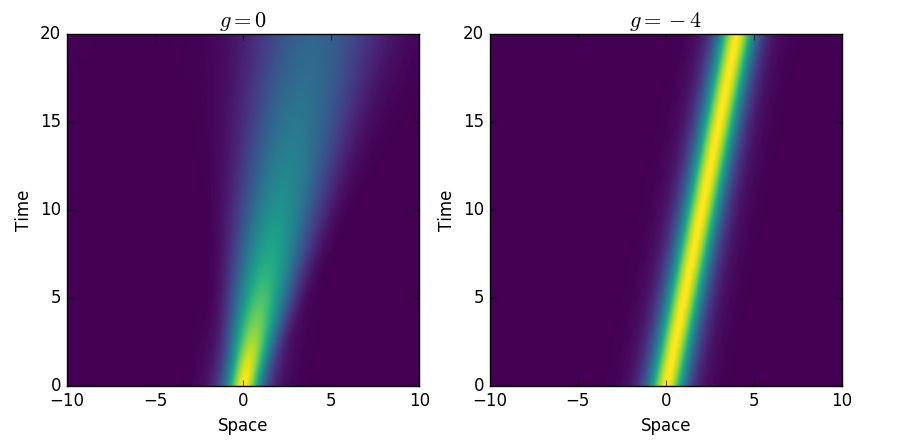
\includegraphics[width=\columnwidth]{milestonepic.png}
\caption{A graph showing the effect of inter-atom interactions $g |\psi|^2$ on a soliton model. The family 
parameter $\zeta = 1$ hence $g=-4$ perfectly confines the soliton with velocity $v=0.2$.}
\label{milestone}
\end{figure}

Since the accuracy was not perfect with $g=-4$, values of $g$ in a small range $\Delta g = 0.01$ either side of the theoretical value were investigated. The accuracy test was run on each, for a space-time box of 2000x2000 points ($x \in [-10,10]$, $t \in [0,2]$) and 6000x6000 points ($x \in [-10,10]$, $t \in [0,6]$). The results are plotted in Fig. \ref{errorsfig}. 

\begin{figure}[h] 
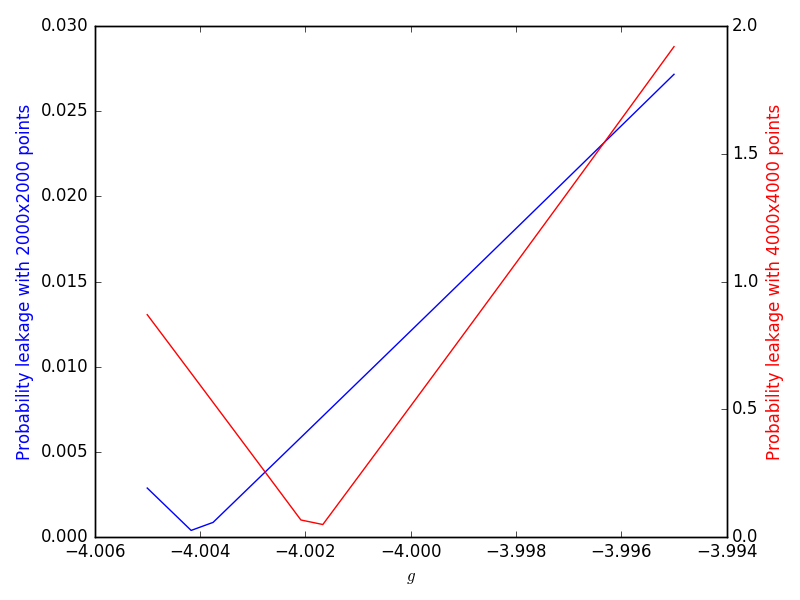
\includegraphics[width=\columnwidth]{errors.png}
\caption{A comparison of the optimal value of $g$, found from the minimum probability leakage, using a discrete space-time grid of 2000x2000 points (blue) compared to 6000x6000 points (magenta). The optimal $g$ value is closer to -4 when space and time more closely approximate a continuum.}
\label{errorsfig}
\end{figure}

As you can see, when the discretisation of space is improved from 2000 points to 6000 points the probability leakage is smaller, for almost every value of $g$ considered. More notably, the interaction parameter with the minimum error in a 2000x2000 box is around $g \approx -4.0025$, whereas for 6000 space points the optimal value is around $g \approx -4.001$. This is significantly closer to the theoretical prediction of $-4$, agreeing with the hypothesis (see section \ref{Intro}) that the slight disagreement with theory is due to the discretisation of space.


%%%%%%%%%%%%%%%%%%%%%%%%%%%%%%%%%%%%%%%%%%%%%%%%%%%%%%

\section{Results and Discussion} \label{Results}

%%%%%%%%%%%%%%%%%%%%%%%%%%%%

\subsection{Collisions}

Two solitons were created at positions symmetric about zero and given equal and opposite velocities to cause them to collide roughly halfway through the time period modelled. The resulting dynamics were plotted for different values of the interaction parameter $g$, two of which are plotted in Fig.\ref{collision}. For small negative values of $g$, the family parameter is small hence the solitons are initially fairly diffuse, since $\zeta$ is inversely proportional to soliton width. These solitons therefore produce a large interference pattern when they collide, but emerge with their velocities and relative phase unchanged. Large negative $g$ values and hence very narrow solitons have counterintuitive collision properties, seeming to 'bounce off' one another when in antiphase. This is due to the wave properties of the condensate and is not indicative of the constituent atoms actually undergoing elastic collisions. 

\begin{figure*}
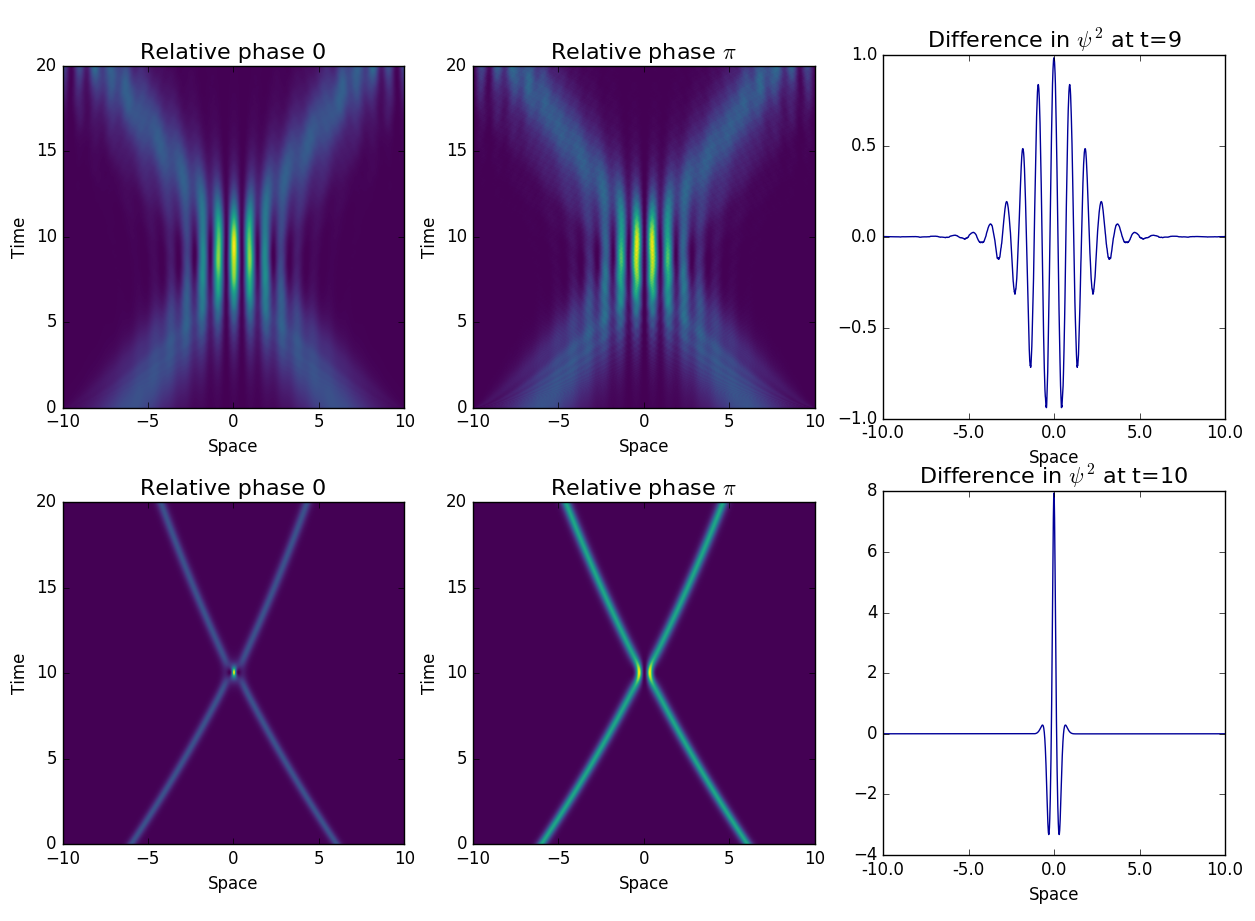
\includegraphics[width=\textwidth]{extensionpic.png}
\caption{A series of graphs showing the collisions of two solitons with speed $|v|=2/3$. Subplots (a)-(c) relate to solitons with $\zeta=0.5$ and subplots (d)-(f) relate to solitons with $\zeta=4$. In plots (a) and (d), the solitons are in phase. In plots (b) and (e) they are in antiphase. Plots (c) and (f) show more clearly the difference between in-phase and antiphase collisions.}
\label{collision}
\end{figure*}

For relative phases of $\pi/2$ and $3\pi/2$ the interference pattern is asymmetric (see Fig.\ref{asymmetric}), retaining the appearance of solitons bouncing off one another but with one soliton heavily weighted in amplitude. 

\begin{figure*}
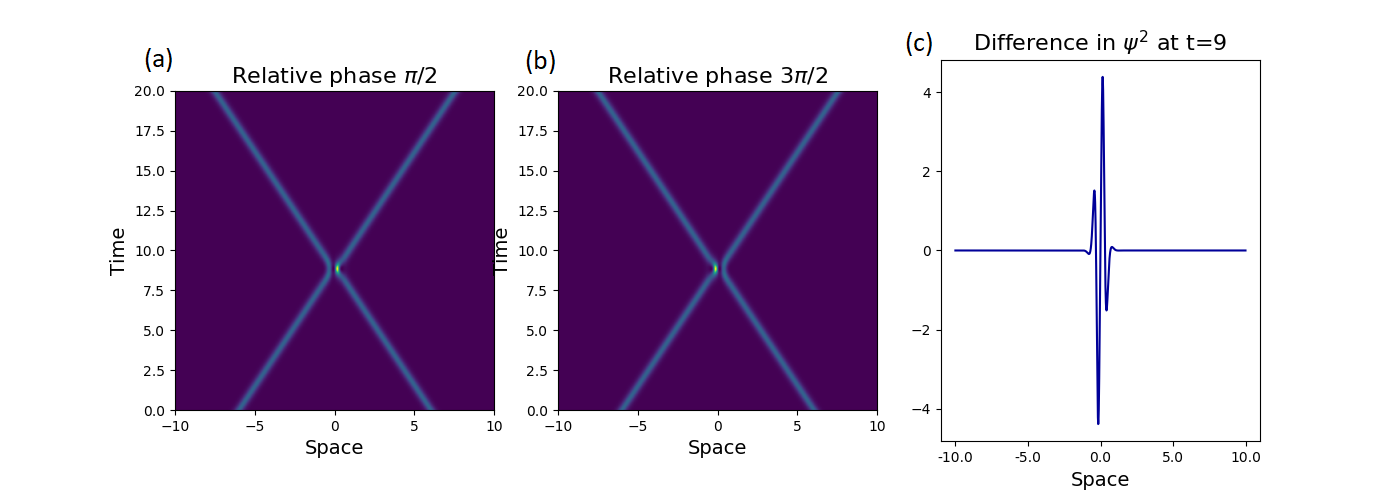
\includegraphics[width=\textwidth]{asymmetrical_collision.png}
\caption{A series of graphs showing the collisions of two solitons with $\zeta=4$ and speed $|v|=2/3$. In subplot (a), the solitons have a relative phase of $\pi/2$. In plot (b) they have a relative phase of $3\pi/2$. Plot (c) shows the difference between these two cases.}
\label{asymmetric}
\end{figure*}

At first glance, the two phase cases for $\zeta=0.5$ (see Fig.\ref{collision} subplots (a) and (b)) look very similar. In reality, where the solitons are in phase at the time of collision there is a central bright fringe in the interference pattern, as opposed to a central dark fringe in the antiphase case. Subplot (c) is included to illustrate this, showing the difference $\psi_0^2 - \psi_{\pi}^2$ at the time of collision. 

When narrow solitons collide (see Fig.\ref{collision} subplots (d) and (e)), the resulting interference resembles a particle-particle interaction, especially in the antiphase case. However, the strong interactions seem to have caused an attractive force between the solitons as evidenced by the final separation of $\Delta x = 9$ compared to the initial separation of $\Delta x=12$. This result is somewhat unexpected as solitons do not usually affect each other even under collisions. It is possible that the solitons were not well-separated so formed a short-lived bound state \cite{Bound}.

%%%%%%%%%%%%%%%%%%%%%%%%%%%%

\subsection{Repeated Collisions}

\begin{figure*}
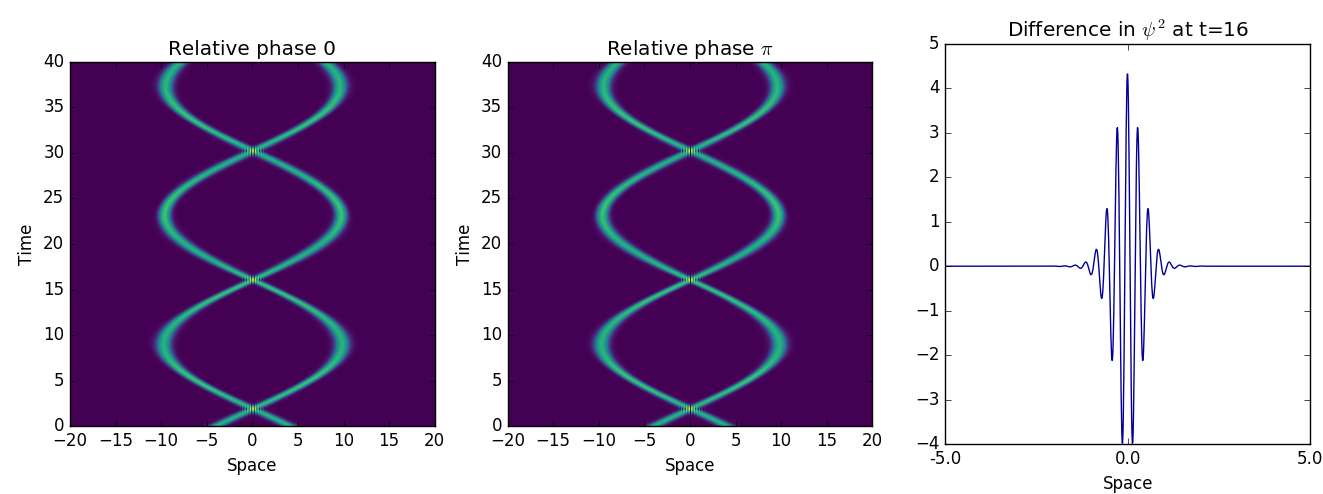
\includegraphics[width=\textwidth]{difference-g7.png}
\caption{A series of graphs showing the repeated collisions of two solitons with $\zeta=7$ and speed $|v|=2$. In subplot (a) the solitons are in phase whilst in subplot (b) they are in antiphase. Plot (c) shows the difference between these two cases.}
\label{repeated}
\end{figure*}

Here a weak axial harmonic confining potential has been introduced with frequency $\omega_x = 2\pi \times 0.25$ Hz. In this case, contrary to the free solitons situation, after a collision the solitons climb a distance up the potential barrier dictated by their momentum and return to collide again. The axial potential preserves the relative phase and velocity of the solitons, allowing perfect periodic motion. However, the introduction of this potential places limits on the range of interaction parameters $g$ which lead to soliton-like behaviour. Observing repeated collisions for a range of values of $g$ and imposing momentum and energy conservation results in a necessary restriction of the interaction parameter to $5 \leq g \leq 13$ in order to retain soliton-like behaviour. 

Fig. \ref{repeated} shows the repeated collisions of two solitons with $\zeta=7$ and speed $|v|=2$ in rescaled units. The data are plotted using a logarithmic colour mapping with a linear cutoff of $|\psi|^2 \leq 0.3$. Subplot (a) shows two solitons colliding in-phase, giving a central density maximum whilst subplot (b) shows the antiphase case with a central minimum. Similarly to the case of a single collision, the difference between these two phase cases is plotted in subplot (c) at a time $t=16$ which corresponds to the solitons' second collision. 

It is important to note that whilst the solitons both undergo a phase shift in each collision, these shifts appear to be such that the phase difference between the two solitons is preserved. This can be seen by closely inspecting each collision in Fig. \ref{repeated} (b) and observing a central density minimum in each case, corresponding to a relative phase of $\pi$. Whilst the preservation of relative phase may seem obvious, if it were not the case it would have impacts on the condensate's stability. It has been observed \cite{Collapse} that BECs containing solitons in antiphase with each other are actually more resistant to collapse than those containing solitons colliding in phase. 

\begin{figure}[h]
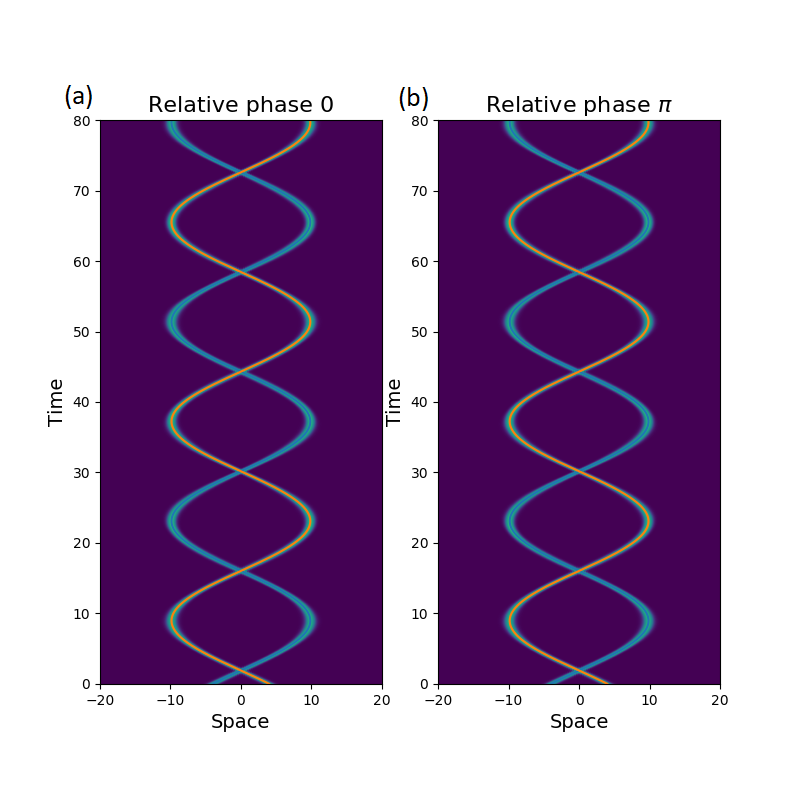
\includegraphics[width=\columnwidth]{repeated-particles.png}
\caption{A set of graphs showing repeated collisions of two solitons with $\zeta=7$ and speed $|v|=2$ with the particle model overlaid. The in-phase and antiphase cases are shown in (a) and (b) respectively. There is no noticeable discrepancy between the wave soliton and particle models in either case for this time period.}
\label{repeated-particles}
\end{figure}

The particle model described in section \ref{Methods} was introduced for repeated soliton collisions. Despite not including soliton-soliton interactions, as you can see in Fig. \ref{repeated-particles} the model has very good agreement with the soliton dynamics predicted by the GPE. If the simulation time period is extended to 200$\tilde{t} = 0.214$ s, small discrepancies start to appear. The wave solitons collide slightly earlier each time than the particle model predicts, which is due to the fact that there is a weak attractive force between solitons which causes them to collide more frequently than if they were under the influence of the confining potential alone. Therefore for typical experimental timescales of less than 0.1 s, the non-interacting particle model is an excellent description of solitons in BECs. 

%%%%%%%%%%%%%%%%%%%%%%%%%%%

\subsection{Three Solitons}

The extension to three solitons supports both regular and chaotic dynamics \cite{Gardiner}. Chaotic behaviour usually arises as a result of two or more of the solitons forming a bound state, as seen in Fig.\ref{chaotic}. When the dynamics are regular, the motion is periodic and the non-interacting particle model agrees very well with the soliton picture (see Fig.\ref{3solitons}). Similarly to the case of two solitons, at later times there is some disagreement between the GPE dynamics and particle dynamics. But after around 400$\tilde{t} = 0.428$ s, the accuracy of the simulation is compromised, with large particle losses in the form of probability leakage; hence over the range of $t$ where the computation is realistic the particle model agrees very well. 

However, the agreement with the particle model breaks down completely on the formation of a bound state in the case where the dynamics are not regular. It has been shown in \cite{Martin} that where the (rather complicated) inter-soliton attractive potential for three solitons is implemented in a particle model, the particle dynamics agree relatively well with the wave dynamics even in chaotic regimes. Clearly the particles cannot be modelled as non-interacting when the soliton interactions are so fundamental to their motion even outside of the localised collisions, which are still clearly observed. However, in this case the particle model is still useful as a visualisation aid to fully appreciate the irregularity of the solitons' motion. 

\begin{figure}[h]
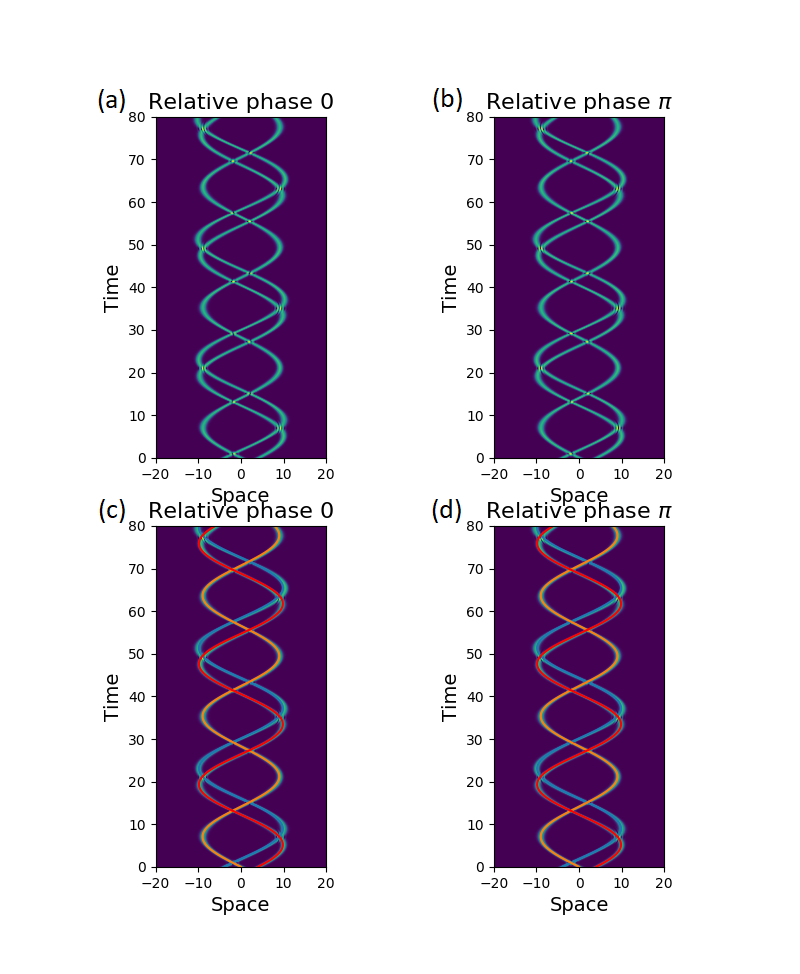
\includegraphics[width=\columnwidth]{3solitons.png}
\caption{Three solitons with equal speeds undergoing collisions with regular periodic dynamics. The in-phase and antiphase cases are both shown. The particle model is overlaid as lines in subplots (c) and (d) and agrees well with both phase cases for this time period.}
\label{3solitons}
\end{figure}

\begin{figure}[h]
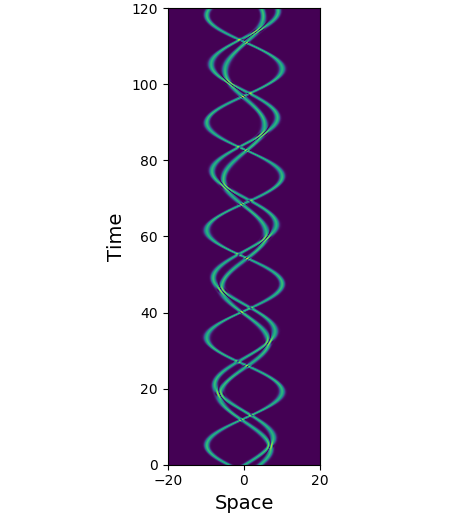
\includegraphics[width=\columnwidth]{chaotic.png}
\caption{Three solitons with speeds 8, 8.15 and 6.28 respectively, undergoing collisions with chaotic dynamics. The particle model is overlaid as lines in subplot (b), and shows that the chaotic soliton behaviour is due to soliton-soliton interactions since the particle dynamics are completely regular.}
\label{chaotic}
\end{figure}

%%%%%%%%%%%%%%%%%%%%%%%%%%%

%%%%%%%%%%%%%%%%%%%%%%%%%%%%%%%%%%%%%%%%%%%%%%%%%%%%%%

\section{Conclusions}

In this project, a method for modelling bright matter-wave solitons in Bose-Einstein condensates was developed and tested, achieving $<0.01\%$ probability leakage. Soliton collisions were investigated for a range of values of the interaction parameter $g$. Good agreement was found with theory, including the observation that colliding solitons in antiphase results in the solitons appearing to bounce off one another. Interference fringes were observed during collisions and the spacing of these had a dependence on the family parameter $\zeta$, which itself depends on $g$. A short-lived bound state was observed when the interactions between atoms were strong. 

A weak harmonic axial confining potential was then introduced for the purpose of observing repeated collisions between solitons. It was observed that the phase difference between two solitons was preserved in subsequent collisions, agreeing with recent experimental findings on the stability of condensates.  

A classical particle model was introduced, as in previous research, but for simplicity the weak inter-soliton potential was set to zero and the temporal limits of this model were investigated. This particle model has excellent agreement with the GPE evolution of solitons when the soliton dynamics are regular and the solitons remain well-separated, over typical experimental timescales. 

Finally, a third soliton was introduced and different relative velocities were investigated to identify cases of periodic and non-periodic motion. The non-interacting particle model had very good agreement with the wave solitons in the case of regular periodic dynamics. But when two or more of the solitons approached closely for an extended period of time, the GPE evolution predicted formation of a bound state which usually led to chaotic dynamics. The particle model implemented here could not reproduce the phenomenon of bound states of solitons, nor of chaos. In these cases, neglecting the weak interaction between solitons is not valid and the inter-soliton potential in section \ref{Intro} must be included. The evolution of solitons as predicted by the GPE is in excellent agreement with theory even in chaotic regimes, though, and the particle model provides a useful contrast when soliton dynamics are chaotic. 


%%%%%%%%%%%%%%%%%%%%%%%%%%%%%%%%%%%%%%%%%%%%%%%%%%%%%%

\begin{thebibliography}{}

\bibitem{Gross} E. P. Gross (1961), "Structure of a quantised vortex in boson systems", \textit{Il Nuovo Cimento} 				\textbf{20}(3) pp. 454-477. 
\bibitem{Pitaevskii}  L. P. Pitaevskii (1961), "Vortex lines in an imperfect Bose gas", \textit{Sov. Phys. JETP.} \textbf{13}(2) 		pp. 451–454.
\bibitem{Bound} N.-C. Panoiu, I. V. Mel’nikov, D. Mihalache, C. Etrich and F. Lederer (1999), "Multiwavelength pulse 			transmission in an optical fibre - Amplifier system", \textit{Phys. Rev.} \textbf{60}(4868). %bound state
\bibitem{Martin} A. D. Martin, C. S. Adams and S. A. Gardiner (2008), "Bright Solitary-Matter-Wave Collisions in a Harmonic 		Trap: Regimes of Soliton-like Behaviour", \textit{Physical Review A} \textbf{77}(1). %particle model 
\bibitem{Transforms} S. Damgaard Hansen, N. Nygaard and K. Mølmer (2012), "Scattering of matter wave solitons on 			localized potentials", arXiv:1210.1681. %transformations of x, t, psi
\bibitem{Cornish} T. Billam, S. Cornish and S. Gardiner (2010), "Realizing bright matter-wave soliton collisions with 				controlled relative phase", \textit{Physical Review A} \textbf{83}(4). %characteristic soliton lengths 
\bibitem{ExpParams} S. L. Cornish et al. (2009), "Quantum reflection of bright matter-wave solitons", \textit{Physica D} 			\textbf{15}(238), following JILA soliton experiments. 
\bibitem{Feshbach} S. Inouye et al. (1998), "Observation of Feshbach resonances in a Bose–Einstein condensate", 				\textit{Nature} \textbf{392} pp. 151-154. 
\bibitem{Gardiner} S. A. Gardiner (2002), "(Quantum) chaos in Bose-Einstein condensates", \textit{Journal of Modern Optics} 	\textbf{49} pp. 1971-1977.
\bibitem{Collapse} L. D. Carr and J. Brand (2004), "Spontaneous Soliton Formation and Modulational Instability in Bose-			Einstein Condensates", \textit{Phys. Rev. Lett.} \textbf{92}(4) 040401. %collapsing BECs

\end{thebibliography} 

%%%%%%%%%%%%%%%%%%%%%%%%%%%%%%%%%%%%%%%%%%%%%%%%%%%%%%

%\section{Appendix} \label{Appendix}

\end{document}